\documentclass{mwart} 
\usepackage[polish]{babel} 
\usepackage[utf8]{inputenc} 
\usepackage{polski} 
\usepackage[T1]{fontenc} 
\usepackage{graphicx}

\usepackage[margin=1cm]{geometry}




\frenchspacing 

\usepackage{indentfirst} 
\title{\Huge{Sprawozdanie z laboratorium nr 4 \\
ALGORYTMY SORTUJĄCE}}
\author{Agnieszka Wiśniewska, nr albumu: 200466}
\date{23.03.2014} 
\begin{document}

\maketitle

\section{Opis zadania\label{wstep}}

Zadaniem do wykonania było przygotowanie programu mierzącego czas wykonywania wybranych algorytmów sortowania. Wyniki jego działań można zobaczyć na wykresach w punkcie \ref{wyniki}.

\section{Wyniki działania programu --- wykresy\label{wyniki}}
\subsection {Sortowanie szybkie (quicksort)}
Jest to wydajny algorytm sortowania działający na zasadzie "Dziel i zwyciężaj" - z tablicy wybiera się element rozdzielający, po czym jest ona dzielona na dwa fragmenty: do początkowego przenoszone są wszystkie elementy nie większe od rozdzielającego, do końcowego wszystkie większe. Następnie sortuje się osobno początkową i końcową część pierwszej tablicy. Rekurencja kończy się, gdy kolejny fragment uzyskany z podziału zawiera pojedynczy element, jako że jednoelementowa tablica nie wymaga sortowania.
\\*\\*
Średnia czasowa złożoność obliczeniowa: O(nlogn)
\begin{figure}[!htp]
\centering
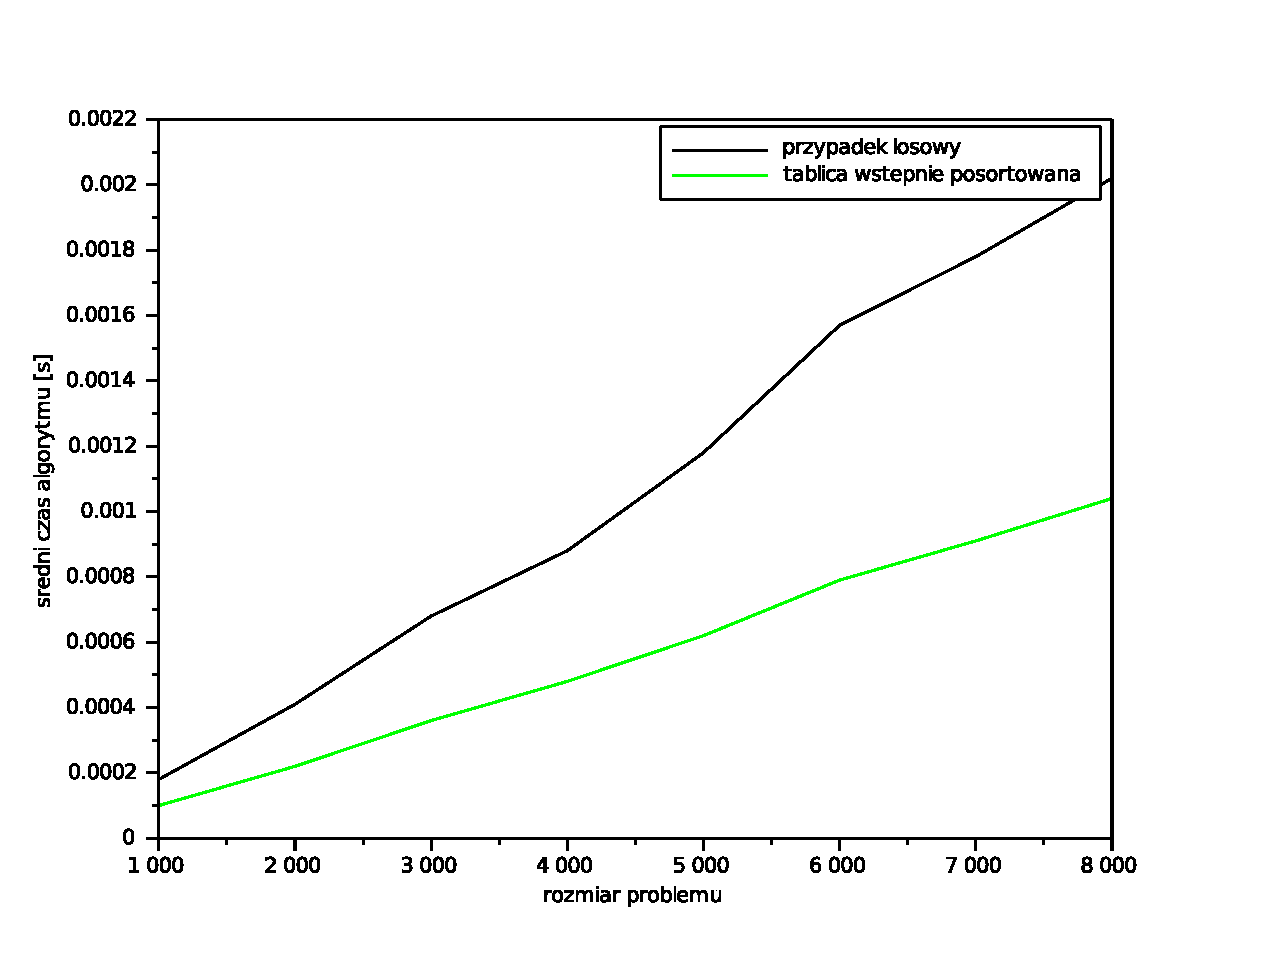
\includegraphics[width=0.8\textwidth]{files/quick.pdf}
\caption{Zależność czasu wykonywania algorytmu od rozmiaru problemu dla sortowania szybkiego. \label{quicksort}} 
\end{figure}


\newpage
\subsection {Sortowanie przez scalanie (mergesort)}
Ten algorytm również działa na zasadzie "dziel i zwyciężaj". Na początku rozdziela się dane na dwie części, sortuje je przez scalanie (chyba, że pozostał już tylko jeden element), aby w końcu połączyć wszystkie podciągi w jeden posortowany ciąg.
\\*\\*
Średnia czasowa złożoność obliczeniowa: O(nlogn)

\begin{figure}[!htp]
\centering
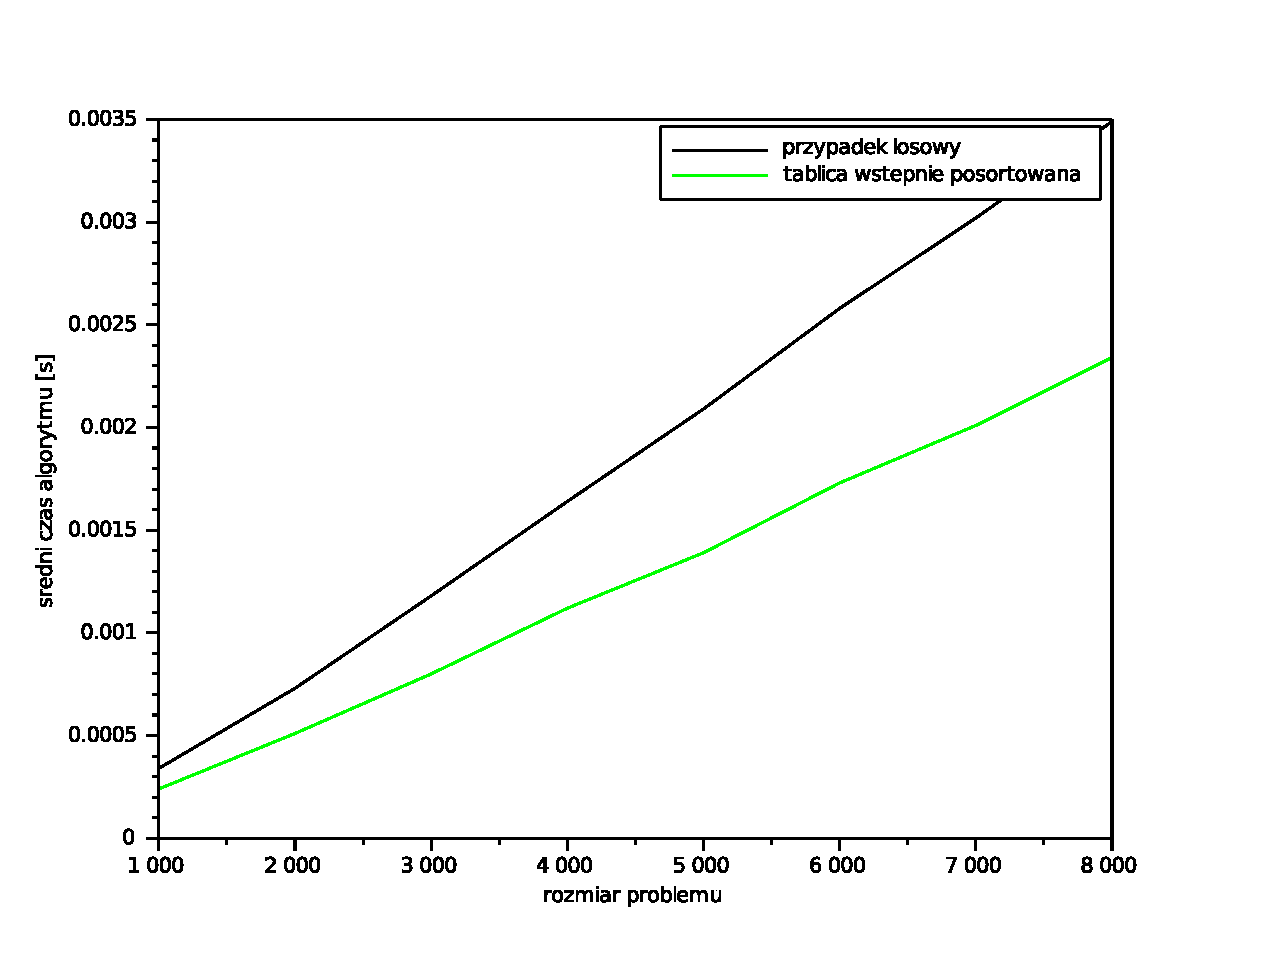
\includegraphics[width=\textwidth]{files/merge.pdf}
\caption{Zależność czasu wykonywania algorytmu od rozmiaru problemu dla sortowania przez scalanie. \label{merge}} 
\end{figure}


\newpage
\subsection {Sortowanie przez kopcowanie (heapsort)}
Niestabilny, lecz szybki i niepochłaniający dużo pamięci algorytm sortowania danych. Działa na podstawie użycia kolejki priorytetowej zaimplementowanej w postaci binarnego kopca zupełnego. Algorytm składa się z dwóch faz - w pierwszej fazie sortowane elementy są reorganizowane w celu utworzenia kopca, w drugiej dokonywane jest właściwe sortowanie.
\\*\\*
Średnia czasowa złożoność obliczeniowa: O(nlogn)

\begin{figure}[!htp]
\centering
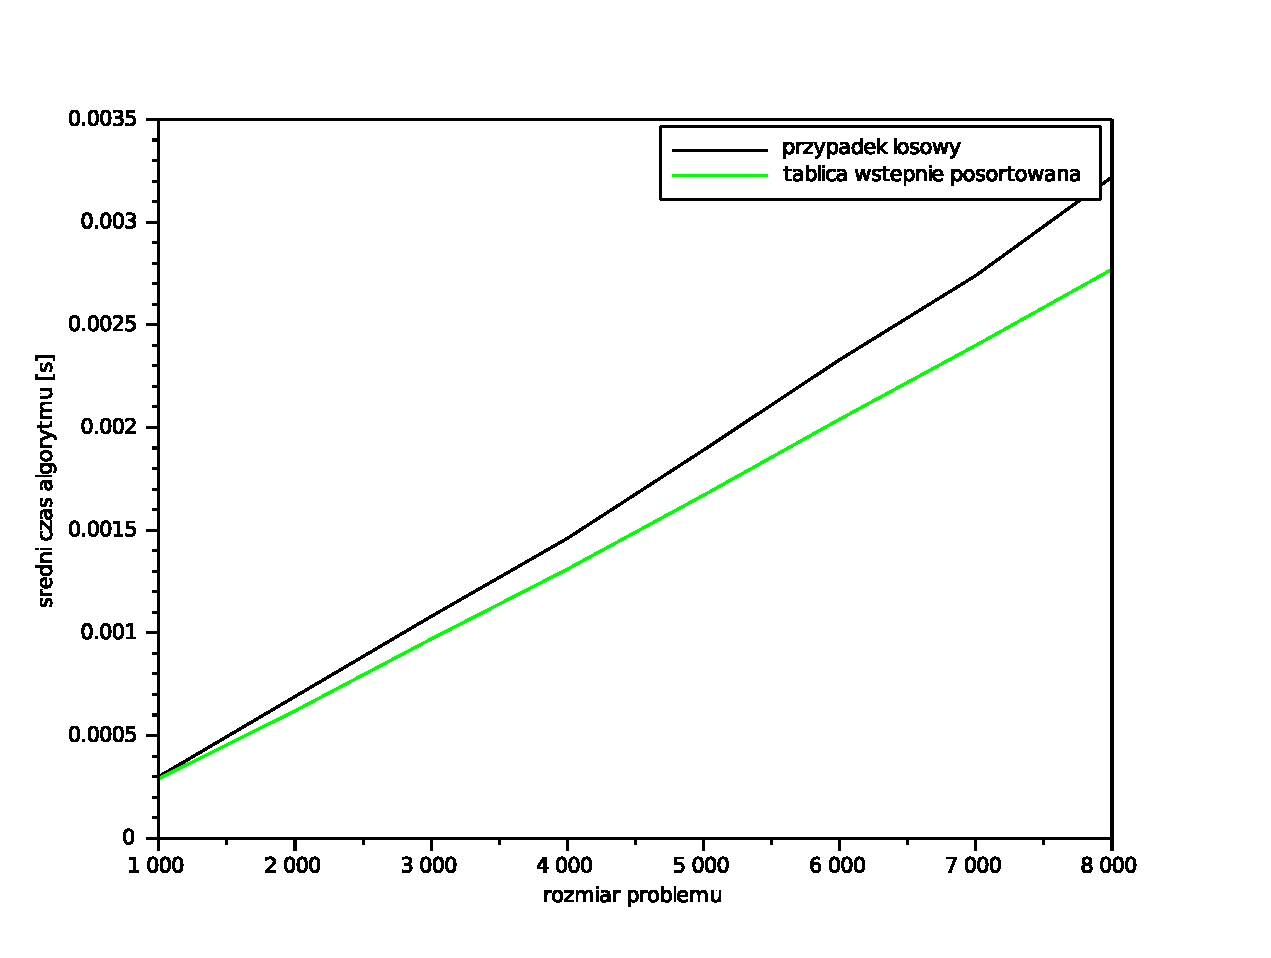
\includegraphics[width=\textwidth]{files/heap.pdf}
\caption{Zależność czasu wykonywania algorytmu od rozmiaru problemu dla sortowania przez kopcowanie. \label{heap}} 
\end{figure}




\section{Wnioski\label{wnioski}}
\begin{itemize}
\item Z powyższych wykresów wynika, że wszystkie trzy przetestowane algorytmy są wydajniejsze dla danych wstępnie posortowanych.
\item Średnia czasowa złożoność obliczeniowa dla testowanych algorytmów wynosi O(nlogn)
\end{itemize}

\section{Załączniki}
\begin{itemize}
\item Dokumentacja z Doxygena "Dokumentacja.pdf"
\end{itemize}

\end{document}
